\documentclass[letterpaper, 11pt, DIV=11]{scrartcl}
\usepackage[utf8x]{inputenc}
\usepackage[T1]{fontenc}
\usepackage{../customlisting}
\usepackage{../customlisting-unicode}
\usepackage[american]{babel}
\usepackage{mathptmx}
\usepackage{graphicx}
\usepackage{microtype}
\usepackage{metalogo}
\usepackage{caption}
\usepackage{hyperref}



\addtokomafont{disposition}{\rmfamily}
\author{\href{https://www.alanshawn.com}{Ziyue ``Alan'' Xiang}}
\title{Typeset Code Listings and Emulate Console Screenshots with \LaTeX\  Beautifully\\ {\small \url{https://github.com/xziyue/latex-beautiful-listings-screenshot}}}
\date{\today}


\newmintinline[texinline]{latex}{frame=none, fontsize=\fontsize{10}{10}}

\newtcblisting{tcbsrccode}[1]{
    tcbcodebasestyle,listing engine=minted, breakable, colback=black!5, boxsep=0pt, colframe=black!30, minted options={linenos,autogobble,breaklines, numbersep=3mm, obeytabs, tabsize=2,fontsize=\fontsize{8}{8}},
    minted language=#1
}

\newenvironment{mylisting}{\medskip\captionsetup{type=listing, labelsep=colon}}{\medskip}
\DeclareCaptionType{lstcap}[Listing][List of Code Listings]

\begin{document}


\pagenumbering{Roman}

\maketitle

\tableofcontents

\clearpage

\pagenumbering{arabic}


\section{Quick Start Guide}

\begin{enumerate}
\item Download \href{https://github.com/xziyue/latex-beautiful-listings-screenshot/blob/master/customlisting.sty}{\rawinline|customlisting.sty|} and place it in your project folder.
\item Load the package with \texinline|\usepackage{customlisting}|.
\item If you are using pdf\LaTeX, make sure to include \texinline|\usepackage[T1]{fontenc}| in the preamble. Otherwise, symbols like \textasciitilde\ may not be displayed correctly.
\end{enumerate}

This package provides the following environments:
\begin{itemize}
\item \rawinline|tcbconsole|, \rawinline|tcbconsole*|
\item \rawinline|tcbcode|, \rawinline|tcbcode*|
\item \rawinline|tcbverbatim|, \rawinline|tcbverbatim*|
\end{itemize}

This package also provides the following commands:
\begin{itemize}
\item \rawinline|tcbinputcode|, \rawinline|tcbinputcode*|
\item \rawinline|tcbinputverbatim|, \rawinline|tcbinputverbatim*|
\end{itemize}

The starred environments/commands offer \emph{unbreakable} listing boxes; while normal ones are \emph{breakable}.



\section{Typeset Source Code Listings}

\begin{itemize}

\item Typeset source code inside \TeX\ files

\begin{tcbsrccode}{text}
\begin{tcbcode}{cpp}
#include <iostream>  
using namespace std; 

int main(){ 
    cout<<"Hello World\n"; 
    return 0; 
} 
\end{tcbcode}
\end{tcbsrccode}
\begin{tcbcode}{cpp}
#include <iostream>  
using namespace std; 

int main(){ 
    cout<<"Hello World\n"; 
    return 0; 
} 
\end{tcbcode}


\item Typeset source code from external source files

\begin{tcbsrccode}{text}
\tcbinputcode*{cpp}{../res/example.cpp}
\end{tcbsrccode}
\tcbinputcode*{cpp}{../res/example.cpp}

\item Inline source code

\begin{tcbsrccode}{text}
\cinline|printf("%s", "some text");|
\pyinline|map(lambda x:x, [1, 2])|
\rawinline|raw value|
\end{tcbsrccode}
\cinline|printf("%s", "some text");|
\pyinline|map(lambda x:x, [1, 2])|
\rawinline|raw value|

\item Declare inline macros for other languages

\begin{tcbsrccode}{text}
\newmintinline[rubyinline]{ruby}{frame=none, fontsize=\fontsize{10}{10}}
\rubyinline|puts 'Hello, world!'|
\end{tcbsrccode}
\newmintinline[rubyinline]{ruby}{frame=none, fontsize=\fontsize{10}{10}}
\rubyinline|puts 'Hello, world!'|

\end{itemize}

\section{Typeset Generic Verbatims}

\begin{itemize}
\item Typeset generic verbatims inside \TeX\ files

\begin{tcbsrccode}{text}
\begin{tcbverbatim}
__________________________  ___
\__    ___/\_   _____/\   \/  /
  |    |    |    __)_  \     / 
  |    |    |        \ /     \ 
  |____|   /_______  //___/\  \
                   \/       \_/
\end{tcbverbatim}
\end{tcbsrccode}
\begin{tcbverbatim}
__________________________  ___
\__    ___/\_   _____/\   \/  /
  |    |    |    __)_  \     / 
  |    |    |        \ /     \ 
  |____|   /_______  //___/\  \
                   \/       \_/
\end{tcbverbatim}


\item Typeset generic verbatims from external files

\begin{tcbsrccode}{text}
\tcbinputverbatim*{../res/wireshark.txt}
\end{tcbsrccode}
\tcbinputverbatim*{../res/wireshark.txt}

\end{itemize}


\section{Typeset Console Screenshots}

Typesetting console screenshots is a bit trickier. By far, it can be done most conveniently on Ubuntu 18.04+. The key is to convert ANSI color codes used by the console into HTML. As it is shown in Figure \ref{fig:ubuntu-conv}, on Ubuntu 18.04+, this can be done simply by selecting the desired region, right click and select ``Copy as HTML''. On other platforms, this should be also doable by dumping the terminal output to a file and using a conversion tool such as \href{https://pypi.org/project/ansi2html/}{\rawinline{ansi2html}}.

\begin{figure}[htpb]
\centering
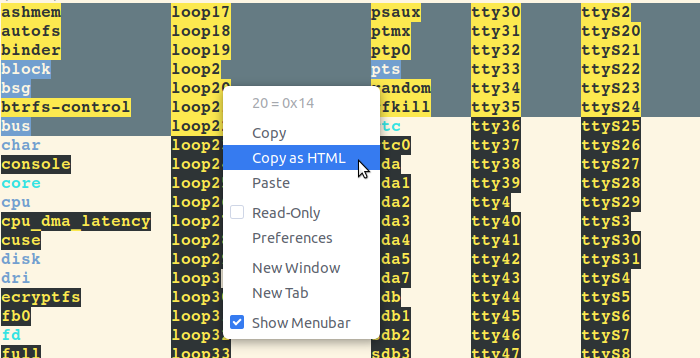
\includegraphics[width=0.6\linewidth]{../res/ubuntu-html}
\caption{Converting terminal output to HTML on Ubuntu 18.04+.}
\label{fig:ubuntu-conv}
\end{figure} 

Generally speaking, one needs to fulfill the following requirements:
\begin{enumerate}
\item Have a way of converting terminal output to HTML.
\item Be able to run the \href{https://github.com/xziyue/latex-beautiful-listings-screenshot/blob/master/html2tex_gui.py}{\rawinline|html2latex|} \LaTeX\ Python script. Currently, the script is dependent on \href{https://pypi.org/project/wxPython/}{\rawinline|wxPython|}, \href{https://pypi.org/project/TexSoup/}{\rawinline|TexSoup|}, \href{https://pypi.org/project/colour/}{colour} and \href{https://pypi.org/project/PyLaTeX/}{\rawinline|PyLaTeX|}. Please note that this software is very primitive and does not support many HTML features.
\end{enumerate}

To typeset this screenshot in \LaTeX, one needs to run \rawinline|html2latex| and paste the HTML in the upper text box. By pressing the ``Convert`` button, the corresponding \LaTeX\ code will appear in the lower text box, as it is shown in Figure \ref{fig:python-html2latex}. The result is shown as below.

\begin{tcbsrccode}{text}
\input{../res/console-dev.txt}
\end{tcbsrccode}
\input{../res/console-dev.txt}

\begin{figure}[htpb]
\centering
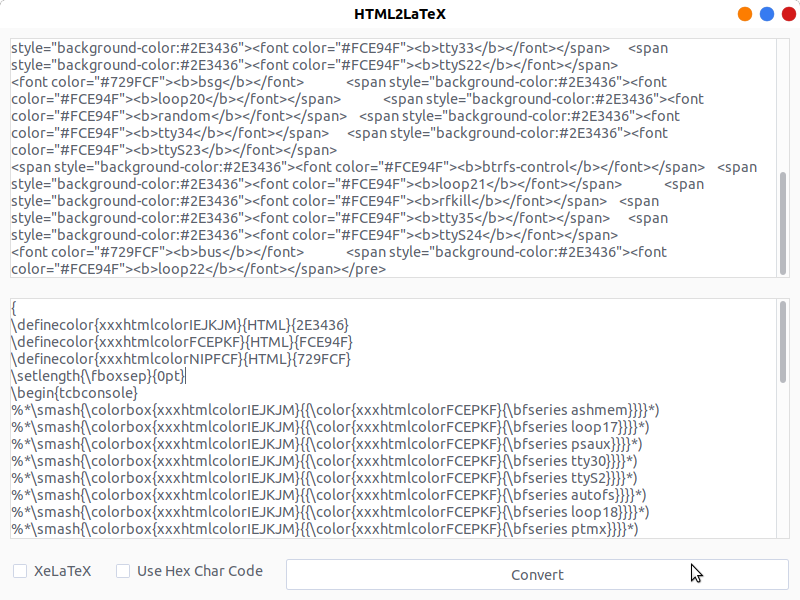
\includegraphics[width=0.7\linewidth]{../res/html2latex}
\caption{Using \rawinline|html2latex| to convert HTML to \LaTeX.}
\label{fig:python-html2latex}
\end{figure} 

Other classic command-line tools, such as \rawinline|emacs|, are supported as well.

\begin{tcbsrccode}{text}
\input{../res/console-emacs.txt}
\end{tcbsrccode}
\input{../res/console-emacs.txt}




\subsection{Unicode Support}

Very frequently, the terminal output contains Unicode characters. For \TeX distribution that supports Unicode input natively (e.g. \XeLaTeX, \LuaLaTeX), this should not be a problem. Just remember to tick the ``XeLaTeX`` check box in \rawinline|html2latex|.


As for the most commonly used pdf\LaTeX, special treatment is needed. The solution is to use the \texinline|\unichar| command provided by loading \texinline|\usepackage[utf8x]{inputenc}|. Therefore, if you are using pdf\LaTeX\ and there is Unicode character inside the terminal output, you should do the following:

\begin{enumerate}
\item Make sure to include \texinline|\usepackage[utf8x]{inputenc}| in your preamble.
\item Put \href{https://github.com/xziyue/latex-beautiful-listings-screenshot/blob/master/customlisting-unicode.sty}{\rawinline|customlisting-unicode.sty|} into your project folder and load it with 

\texinline|\usepackage{customlisting-unicode}|.
\item In \rawinline|html2latex|, make sure ``XeLaTeX`` is unchecked.
\end{enumerate}

A pdf\LaTeX\ example is shown as below. 

\begin{tcbsrccode}{text}
\input{../res/console-unicode.txt}
\end{tcbsrccode}
\input{../res/console-unicode.txt}

However, keep in mind that \textbf{this Unicode support is extremely limited}: many characters are simply unavailable in pdf\LaTeX. Many packages are not compatible with \texinline|\usepackage[utf8x]{inputenc}|. One most notable example is \rawinline|biblatex|. Therefore, for better Unicode support, one should use \XeLaTeX\ or \LuaLaTeX.

\section{Add Captions}

To support captions, one needs to load the \rawinline|caption| package in the preamble and add some related definitions. 

\begin{tcbsrccode}{latex}
\usepackage{caption}

\newenvironment{mylisting}{\medskip\captionsetup{type=listing, labelsep=space}}{\medskip}
\DeclareCaptionType{lstcap}[Listing][List of Code Listings]
\end{tcbsrccode}

This allows one to add caption to code listings with the following code. The ``List of Code Listings'' can be generated with \texinline|\listoflstcaps|.

\begin{tcbsrccode}{text}
\begin{mylisting}
\begin{tcbcode*}{julia}
function quadratic2(a::Float64, b::Float64, c::Float64)
    # unlike other languages 2a is equivalent to 2*a
    # a^2 is used instead of a**2 or pow(a,2)
    sqr_term = sqrt(b^2-4a*c)
    r1 = quadratic(a, sqr_term, b)
    r2 = quadratic(a, -sqr_term, b)
    # multiple values can be returned from a function using tuples
    # if the return keyword is omitted, the last term is returned
    r1, r2
end
\end{tcbcode*}
\end{mylisting}
\listoflstcaps
\end{tcbsrccode}

\begin{mylisting}
\begin{tcbcode*}{julia}
function quadratic2(a::Float64, b::Float64, c::Float64)
    # unlike other languages 2a is equivalent to 2*a
    # a^2 is used instead of a**2 or pow(a,2)
    sqr_term = sqrt(b^2-4a*c)
    r1 = quadratic(a, sqr_term, b)
    r2 = quadratic(a, -sqr_term, b)
    # multiple values can be returned from a function using tuples
    # if the return keyword is omitted, the last term is returned
    r1, r2
end
\end{tcbcode*}
\captionof{lstcap}{Some random Julia function.}
\end{mylisting}
\listoflstcaps
\end{document}